% 中心对称示意：△ABC 绕 O 旋转 180° 得 △A'B'C'
\documentclass[tikz,border=4pt]{standalone}
\usepackage{ctex}
\usepackage{amsmath}
\usetikzlibrary{calc, decorations.markings}
\begin{document}
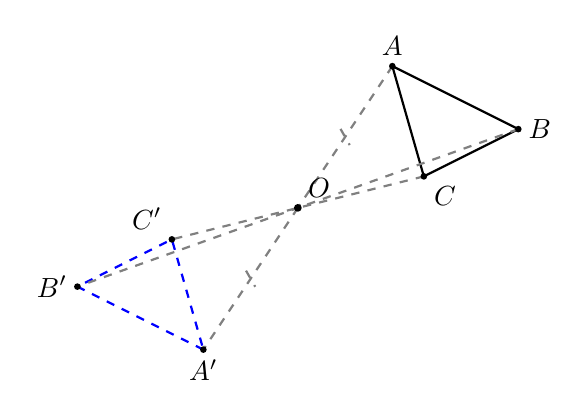
\begin{tikzpicture}[scale=1.0, thick,
  tickone/.style={postaction={decorate, decoration={markings,
    mark=at position 0.5 with {\draw (-1.5pt,-3pt) -- (1.5pt,3pt);}}}}]
  \coordinate (O) at (0,0);
  \coordinate (A) at (1.2, 1.8);
  \coordinate (B) at (2.8, 1.0);
  \coordinate (C) at (1.6, 0.4);
  \coordinate (Ap) at (-1.2, -1.8);
  \coordinate (Bp) at (-2.8, -1.0);
  \coordinate (Cp) at (-1.6, -0.4);

  \draw (A) -- (B) -- (C) -- cycle;
  \draw[blue, dashed] (Ap) -- (Bp) -- (Cp) -- cycle;

  \draw[gray, dashed, tickone] (A) -- (O);
  \draw[gray, dashed, tickone] (O) -- (Ap);
  \draw[gray, dashed] (B) -- (Bp);
  \draw[gray, dashed] (C) -- (Cp);

  \fill (O) circle (1.4pt);
  \fill (A) circle (1.2pt); \fill (B) circle (1.2pt); \fill (C) circle (1.2pt);
  \fill (Ap) circle (1.2pt); \fill (Bp) circle (1.2pt); \fill (Cp) circle (1.2pt);

  \node[above right] at (O) {$O$};
  \node[above] at (A) {$A$};
  \node[right] at (B) {$B$};
  \node[below right] at (C) {$C$};
  \node[below] at (Ap) {$A'$};
  \node[left] at (Bp) {$B'$};
  \node[above left] at (Cp) {$C'$};
\end{tikzpicture}
\end{document}
